%!TEX TS-program = xelatex
\documentclass[mathserif, aspectratio=169]{beamer}

\usetheme{Warsaw}
\usetheme[progressbar=frametitle]{metropolis}
\usepackage{kotex}
\usepackage{ragged2e}

\usepackage{amsmath}
\usepackage{graphics}
\usepackage{setspace}
\usepackage{wrapfig}

\title{인터넷 기사의 댓글 속 혐오 양상에 대하여}
\setbeamerfont{title}{series=\bfseries}

\author{20205178 박~~현\hfill 인공지능 알고리즘을 이용한 사회과학연구 -- 기말 프로젝트}
\setbeamerfont{author}{size=\scriptsize, series=\bfseries}
\institute{}
\date{}

\setbeamertemplate{navigation symbols}{}
% \setbeamerfont{frametitle}{series=\bfseries,parent=structure}

\setbeamertemplate{itemize/enumerate body begin}{\normalsize}
\setbeamertemplate{itemize/enumerate subbody begin}{\footnotesize}
\setstretch{1.25}



\begin{document}
\frame{\titlepage}
\metroset{sectionpage=none}
\metroset{block=fill}

\section{주제 선정 이유}
\begin{frame}
    \frametitle{주제 선정 이유}
    \justifying
    최근 온 $\cdot$ 오프라인 상에서의 혐오가 사회적 문제로 떠오르고 있다.
    이에 수 년간의 인터넷 기사 댓글을 수집하여 Korean UnSmile Dataset에서 제공하는 인공지능 모델을
    이용하여 각 댓글에 해당하는 혐오 분류를 찾아 이들에 대한 분포 및 양상을 군집화 및 회귀를 진행하고자 한다.
\end{frame}
\section{알고리즘 적용 과정}
\begin{frame}
    \frametitle{사용한 패키지}
    \textbf{[ R Packages ]}
    \begin{description}[labelwidth=3cm]
        \item [future:] Unified Parallel and Distributed Processing in R for Everyone
        \item [future.apply:] Apply Function to Elements in Parallel using Futures
        \item [reticulate:]  Interface to `Python'
        \item [rvest:] Easily Harvest (Scrape) Web Pages
        \item [tidyverse:] Easily Install and Load the `Tidyverse'
        % \item [reshape2:] Flexibly Reshape Data: A Reboot of the Reshape Package
    \end{description}
    ~\\
    \textbf{[ Python Libraries ]}
    \begin{description}[labelwidth=3cm]
        \item [Hugging Face:] Datasets, Transformers.
        \item [Pandas:] Python Data Analysis Library
    \end{description}
\end{frame}
\begin{frame}{자료 수집}

    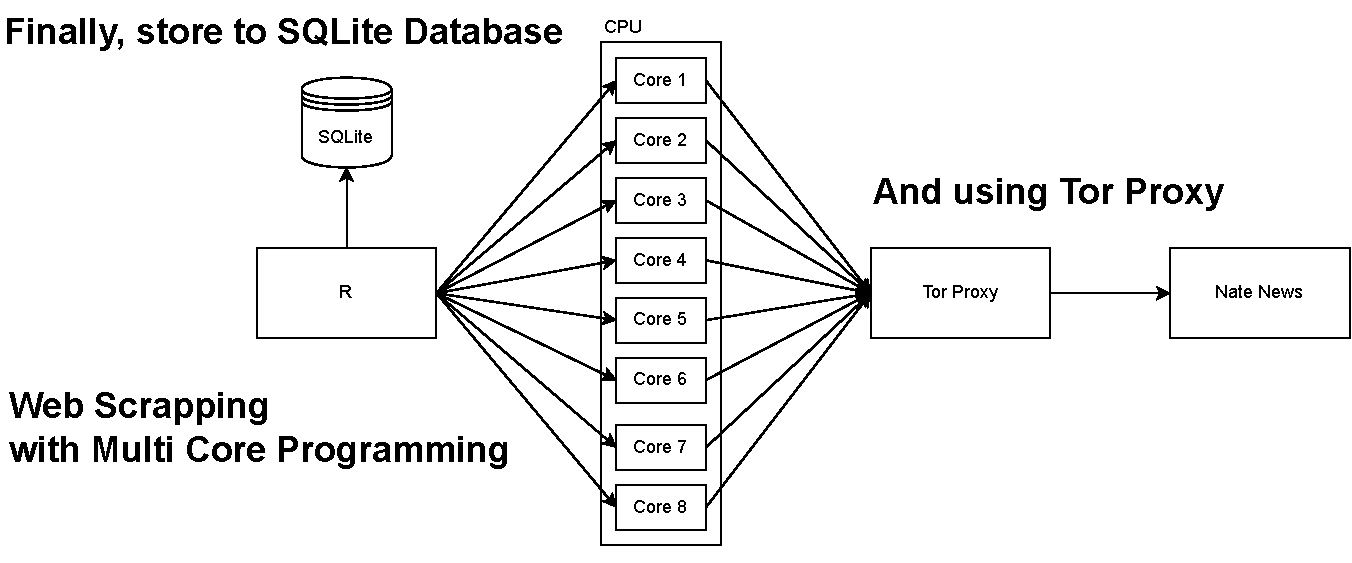
\includegraphics[width = \linewidth]{images/data_scrap.pdf}
\end{frame}
\begin{frame}{테이블 구조}
    \begin{columns}
        \begin{column}{0.5\linewidth}
            
        \end{column}
        \begin{column}{0.5\linewidth}
            테이블 구조는 
        \end{column}
    \end{columns}
\end{frame}
\section{함의}
\end{document}